% !TeX encoding = UTF-8
% !TeX spellcheck = en_US
\documentclass[11pt,a4paper,final]{article}
\usepackage[utf8x]{inputenc}
\usepackage{lmodern}
\usepackage{hyperref}
\usepackage{tikz}
\usepackage{tikz-dsp}
\usetikzlibrary{decorations.pathreplacing}
\usepackage{amsmath}
\author{Matthieu Guerquin-Kern, ENSEA}
\date{\today}
\title{Signal Quality in Multi Stage Sample Rate Converters}
\begin{document}
\maketitle

\begin{abstract}
The purpose of this document is to evaluate the impact that the multi-stage 
implementation of a sample rate converter might have on signal quality.
\end{abstract}

\section{Context}

\subsection{Single Stage Sample Rate Converter}

A synchronous sample rate converter (SRC) can be described by the cascade of an 
upsampler, a filter, and a downsampler.

\begin{center}
\begin{tikzpicture}
\node[dspnodeopen,dsp/label=above] (e0) {$F_\text{in}$};
\node[dspsquare,right=of e0] (e1) {$\upsamplertext{L}$};
\node[dspfilter,right=of e1] (e2) {$H(z)$};
\node[dspsquare,right=of e2] (e3) {$\downsamplertext{M}$};
\node[dspnodeopen,right=of e3,dsp/label=above] (e4) 
{$F_\text{out}$};
\foreach \i [evaluate=\i as \j using int(\i+1)] in {0,1,2,3} {
	\draw[dspconn] (e\i) -- (e\j);
}
\end{tikzpicture}
\end{center}
In the above block diagram, the SRC will change the signal from a rate 
$F_\text{in}$ to a rate $F_\text{out}$ under the constraint that 
$L\cdot F_\text{in}=M\cdot F_\text{out}$ with $L$ and $M$ integers. The linear 
shift invariant filter $H$ plays two roles: interpolating and anti-aliasing 
(sensible only if $M>L$). Therefore, in order to ensure a minimal distortion on 
the signal, one wants the filter as close as possible to a low-pass with cutoff 
pulsation $\omega_c=\pi/\max(L,M)$ and $H(1)=M$. 

\subsection{Multi Stage Sample Rate Converter}
Let us consider the following factorizations
\[L = \prod_{i=1}^N L_i \text{ and }M = \prod_{i=1}^N M_i,\]
where some $L_i$ or $M_i$ might equal $1$ but with $M_i$ ad $L_j$ relatively 
prime $\forall i,j$. Then, we can consider decomposing the SRC into $N$ 
multiple stages of the same form.
\begin{center}
\begin{tikzpicture}
\node[dspnodeopen,dsp/label=above] (e0) {$F_\text{in}$};
\node[dspsquare,right=of e0,xshift=-.7cm] (e1) {$\upsamplertext{L_1}$};
\node[dspfilter,right=of e1,xshift=-.7cm,minimum width=1cm] (e2) {$H_1$};
\node[dspsquare,right=of e2,xshift=-.7cm] (e3) {$\downsamplertext{M_1}$};
\node[dspsquare,right=of e3,xshift=-.7cm] (e4) {$\upsamplertext{L_2}$};
\node[dspfilter,right=of e4,xshift=-.7cm,minimum width=1cm] (e5) {$H_2$};
\node[dspsquare,right=of e5,xshift=-.7cm] (e6) {$\downsamplertext{M_2}$};
\node[dspsquare,right=of e6] (e7) {$\upsamplertext{L_N}$};
\node[dspfilter,right=of e7,xshift=-.7cm,minimum width=1cm] (e8) {$H_N$};
\node[dspsquare,right=of e8,xshift=-.7cm] (e9) {$\downsamplertext{M_N}$};
\node[dspnodeopen,right=of e9,dsp/label=above,xshift=-.7cm] (e10) 
{$F_\text{out}$};
\foreach \i [evaluate=\i as \j using int(\i+1)] in {0,1,...,5} {
	\draw[dspconn] (e\i) -- (e\j);
}
\foreach \i [evaluate=\i as \j using int(\i+1)] in {7,8,9} {
	\draw[dspconn] (e\i) -- (e\j);
}
\draw[thick,dashed,-latex] (e6)--(e7);
\draw [decorate,decoration={brace,amplitude=10pt},xshift=-4pt,yshift=0pt]
(e3.south east)--(e1.south west) node [black,midway,below,yshift=-3mm] 
{stage 1};
\draw [decorate,decoration={brace,amplitude=10pt},xshift=-4pt,yshift=0pt]
(e6.south east)--(e4.south west) node [black,midway,below,yshift=-3mm] 
{stage 2};
\draw [decorate,decoration={brace,amplitude=10pt},xshift=-4pt,yshift=0pt]
(e9.south east)--(e7.south west) node [black,midway,below,yshift=-3mm] 
{stage $N$};
\end{tikzpicture}
\end{center}

Since the $L_i$ and $M_j$ are relatively prime, the two structures are 
equivalent provided that
\begin{equation}\label{eq1}
H(z) = \prod_{i=1}^{N}H_i\left(z^{\tilde{L}_i\cdot 
\tilde{M}_{N-i+1}}\right),
\end{equation}
with the notations $\tilde{L}_i$ and $\tilde{M}_i$ stand for 
$\prod_{k=i+1}^NL_k$ and $\prod_{k=i+1}^NM_k$ if $i<N$, and 
$\tilde{L}_N=\tilde{M}_N=1$.

For the design of the filters $H_i$, one can apply the constraints previously 
seen: low-pass with cutoff pulsation $\omega_c=\pi/\max(L_i,M_i)$ and 
$H_i(1)=M_i$. Then, the question is ``how should organize the stages in order 
to have a minimal impact on signal quality?'' In other words, ``How to sort 
the sequences $L_i$ and $M_i$ in order to have $H$ be the closest to a 
low-pass with cutoff pulsation $\omega_c=\pi/\max(L,M)$''?
\footnote{From \eqref{eq1}, one sees that $H(1)=M$ is not a big deal.}

\section{Simple Example}

In this example, we consider the case where $L=9$, $M=8$ and $N=2$. Since, 
$L_1=L_2=3$, we result in two possible implementations of a dual stage SRC.

\subsection{Case $M_1=2$ and $M_2=4$}

\begin{center}
\begin{tikzpicture}
\node[dspnodeopen,dsp/label=above] (e0) {$F_\text{in}$};
\node[dspsquare,right=of e0] (e1) {$\upsamplertext{3}$};
\node[dspfilter,right=of e1,xshift=-.3cm,minimum width=1cm] (e2) {$H_1$};
\node[dspsquare,right=of e2,xshift=-.3cm] (e3) {$\downsamplertext{2}$};
\node[dspsquare,right=of e3,xshift=-.3cm] (e4) {$\upsamplertext{3}$};
\node[dspfilter,right=of e4,xshift=-.3cm,minimum width=1cm] (e5) {$H_2$};
\node[dspsquare,right=of e5,xshift=-.3cm] (e6) {$\downsamplertext{4}$};
\node[dspnodeopen,right=of e6,dsp/label=above] (e7) 
{$F_\text{out}$};
\foreach \i [evaluate=\i as \j using int(\i+1)] in {0,1,...,6} {
	\draw[dspconn] (e\i) -- (e\j);
}
\end{tikzpicture}
\end{center}
The cutoff frequencies of $H_1$ and $H_2$ are $\pi/3$ and $\pi/4$, respectively.
We have $H(z)=H_1(z^3)H_2(z^2)$. As the following plot shows, there should be 
no problem :
\begin{itemize}
\item outside of low frequencies, the filters act on different 
frequency bands,
\item the resulting cutoff pulsation is $\pi/9$ as expected.
\end{itemize}

\begin{center}
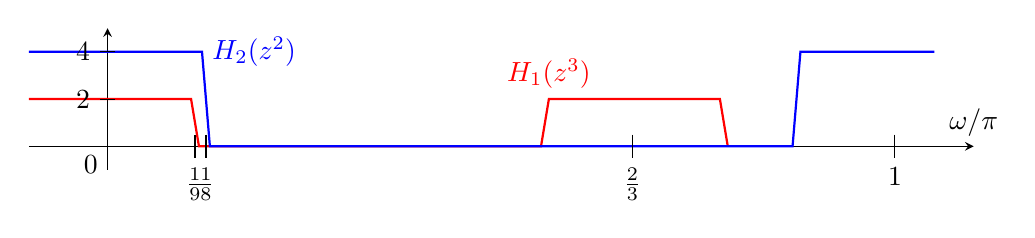
\begin{tikzpicture}[>=stealth,x=10cm,y=3mm]
\draw[->] (-.1,0)--(1.1,0) node[above]{$\omega/\pi$};
\draw[->] (0,-1)--(0,5);
\draw[red,thick] (-.1,2)--({1/9-.005},2) 
--++(.01,-2)--({5/9-.005},0)--++(0.01,2)node[above]{$H_1(z^3)$}--++({2/9-.005},0)--++(.01,-2););
\draw[blue,thick] 
(-.1,4)--({1/8-.005},4)node[right]{$H_2(z^2)$}--++(.01,-4)--({7/8-.005},0) 
--++(0.01,4)--(1.05,4);
\draw (1/9,.5)--++(0,-1) node[below] {$\frac{1}{9}$};
\draw (1/8,.5)--++(0,-1) node[below] {$\frac{1}{8}$};
\draw (2/3,.5)--++(0,-1) node[below] {$\frac{2}{3}$};
\draw (1,.5)--++(0,-1) node[below] {$1$};
\draw (.01,2)--++(-.02,0) node[left] {$2$};
\draw (.01,4)--++(-.02,0) node[left] {$4$};
\node[below left] at (0,0) {$0$};
\end{tikzpicture}
\end{center}

\subsection{Case $M_1=4$ and $M_2=2$}
\begin{center}
\begin{tikzpicture}
\node[dspnodeopen,dsp/label=above] (e0) {$F_\text{in}$};
\node[dspsquare,right=of e0] (e1) {$\upsamplertext{3}$};
\node[dspfilter,right=of e1,xshift=-.3cm,minimum width=1cm] (e2) {$H_1$};
\node[dspsquare,right=of e2,xshift=-.3cm] (e3) {$\downsamplertext{4}$};
\node[dspsquare,right=of e3,xshift=-.3cm] (e4) {$\upsamplertext{3}$};
\node[dspfilter,right=of e4,xshift=-.3cm,minimum width=1cm] (e5) {$H_2$};
\node[dspsquare,right=of e5,xshift=-.3cm] (e6) {$\downsamplertext{2}$};
\node[dspnodeopen,right=of e6,dsp/label=above] (e7) 
{$F_\text{out}$};
\foreach \i [evaluate=\i as \j using int(\i+1)] in {0,1,...,6} {
	\draw[dspconn] (e\i) -- (e\j);
}
\end{tikzpicture}
\end{center}

The cutoff frequencies of $H_1$ and $H_2$ are $\pi/4$ and $\pi/3$, respectively.
We have $H(z)=H_1(z^3)H_2(z^4)$. As the following plot shows, the situation is 
now more complicated because
\begin{itemize}
\item the filters share common frequency intervals in 
high frequencies.
\item the resulting cutoff pulsation $\pi/12$ is lower than expected.
\end{itemize}
 
\begin{center}
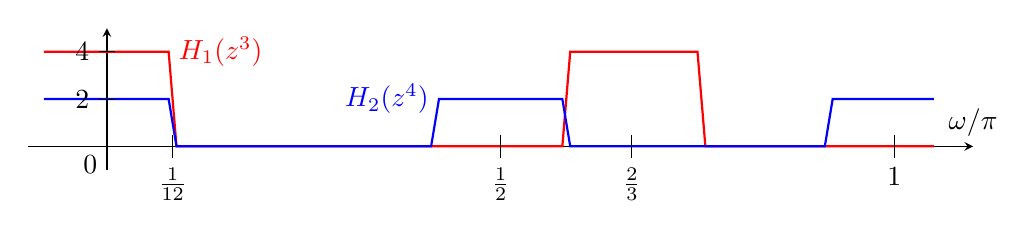
\begin{tikzpicture}[>=stealth,x=10cm,y=3mm]
\draw[->] (-.1,0)--(1.1,0) node[above]{$\omega/\pi$};
\draw[->] (0,-1)--(0,5);
\draw[red,thick] (-.08,4)--({1/12-.005},4) node[right]{$H_1(z^3)$}
--++(.01,-4)--({7/12-.005},0)--++(0.01,4)--++({1/6-.005},0)--++(.01,-4)--(1.05,0);
\draw[blue,thick] (-.08,2)--({1/12-.005},2)--++(.01,-2)--({5/12-.005},0)
--++(0.01,2)node[left]{$H_2(z^4)$} 
--({7/12-.005},2)--++(0.01,-2)--({11/12-.005},0)--++(.01,2)--(1.05,2);
\draw (1/12,.5)--++(0,-1) node[below] {$\frac{1}{12}$};
\draw (1/2,.5)--++(0,-1) node[below] {$\frac{1}{2}$};
\draw (2/3,.5)--++(0,-1) node[below] {$\frac{2}{3}$};
\draw (1,.5)--++(0,-1) node[below] {$1$};
\draw (.01,2)--++(-.02,0) node[left] {$2$};
\draw (.01,4)--++(-.02,0) node[left] {$4$};
\node[below left] at (0,0) {$0$};
\end{tikzpicture}
\end{center}

\end{document}